\chapter{Further work on the model}
\label{secondPhaseOfModelingCyberInsurance} 

So far our model have only considered the effects of direct connections, but in this part we will introduce the effects of indirect connections. When a node connects to a new node, the change in payoff is not just a fixed variable as earlier, but also dependent on the connections already established by the other node.

In the earlier model network effects the nodes experiences, arises from their neighbours only. I.e. when a node establish a connection the change in utility is only dependent on fixed variables, and non dependent of the rest of the network.
In the previous models the utility for each node where only affected by direct variables such as $\beta$. In a real world scenario a node will be strongly affected by network externalities. Our idea is based on the paper from Jackson and Wolinsky \cite{jackson1996strategic} and a network formation game in \cite{jackson2005survey}. 

\section{The connection game}
We consider a connection game where the network effects are dependent on the whole network.  Meaning, in addition to the benefit from the direct connection, a node will also benefit from "the friends of the friend", and "the friends of the friends of the friend" etc. This is achieved by letting the payoff be calculated relative to the distance between the nodes. The network externality $\beta$ is now dependent on the number of hops to the node e.g. the benefit of a direct connection is $\beta$, the benefit of a friend of a friend is $\beta^2$ etc. We want the benefit to be decreasing with the distance, so we need this limitation: $0<\beta<1$ on $\beta$. 

\begin{figure}[h]
\centering
  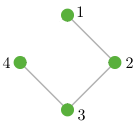
\includegraphics[width=0.2\linewidth]{../Figures/connectionGame.png}
  \caption{\label{fig:connectionGame} Four nodes interconnected with each other.}
\end{figure}
lets consider the network shown in \ref{fig:connectionGame}. Node 1 in the network will get a benefit of $\beta+\beta^{2}+\beta^{3}$ by having the connection with node 2. For this network to make sense, it is important to also include some cost of having direct connections. This is done as in earlier models, every node pay a cost for direct connections, but no cost for indirect connections. Thus the total payoff for a node is:

\begin{equation}
\sum_{j\neq i}^{} \beta_{ij}^{d(ij)} - \sum_{j:ij\in g}^{} {c}_{ij}, 
\label{connecetionGame}
\end{equation}

where $d(ij)$ represents the shortest path between node $i $ and node $j $, and ${c}_{ij}$ represents node i's cost of establishing a link between the two nodes. To simplify the model we choose a symmetric connection process where $\beta$ and $c$ is set to a fixed global value. 

In the paper \cite{jackson1996strategic}, they analyze the stability and efficiency of a network like this. An efficient network means ending up with a network where the sum of every nodes payoff is maximized. The optimal network is of course both efficient and stable, but as we shall see there are some conflicts between efficiency and stability. In the paper they found that an efficient network is:
\begin{enumerate}
\item \textit{a complete graph $g^N$ if $c<\beta - \beta^2$,}
\item \textit{a star encompassing every node if $\beta - \beta^2 < c < \beta + \frac{(N-2)}{2}\beta^2$,}
\item \textit{an empty network(no links) if $\beta + \frac{(N-2)}{2}\beta^2 < c$.}
\end{enumerate}

Proposition 1, says that when the cost of insuring a link is low, it would be more beneficial for every node, to have a direct connection to another node, compared to an indirect connection.
Proposition 3, when the insurance cost is high, it is best to not have any connections at all.

The most efficient structure is created in the intermediate cost of insuring links, and ends up in a star structure which encompasses every node. A star structure have the characteristics of minimizing the average path length and uses the minimum number of links($N-1$) required for including every node to the network. 
Indisputable this structure provides the highest overall payoff for the network, but this network is not necessarily stable, as we will show later on.

\subparagraph{Pairwise stability:(HVERTFALL ISH )}
A graph is pairwise stable if:
 \begin{enumerate}
\item \textit{No node want to delete a link he is involved in.}
\item \textit{If there exists a node who want to add a link, then the node on the other end of the link do not want to establish this link.}
\end{enumerate} 
The limitations of pairwise stability is that we only consider one link and one pair of nodes at a time.


When analyzing the stability of the network, by using pairwise stability, Jackson and Wolinsky found four different conditions of stability:

\begin{enumerate}
\item \textit{a pairwise stable network consists of at most one (non-empty) component,}
\item \textit{if $c<\beta - \beta^2$, the unique pairwise stable network will be a complete graph $g^N$, }
\item \textit{if $\beta - \beta^2 <c < \beta $, a star encompassing every node will be pairwise stable, although not necessarily the unique pairwise stable graph,}
\item \textit{if $\beta < c$ , any pairwise stable network which is nonempty is such that each player has at least two links and thus be inefficient. }
\end{enumerate}
We see that the stability condition 2, is the same as the efficiency condition 1, and thus if this condition is fulfilled, the network is both stable and efficient. 
Condition 3 shows us why the efficient star network is not necessarily  stable. If $\beta \geq c <   \beta + \frac{(N-2)}{2}\beta^2$ then the efficient network will be a star, but it is not stable.

It should be noticed that it is more beneficial for a node to operate as a leaf node compared to being a center node, due to the cost of direct connection. In a star structure, a leaf node will only have to pay the cost of the link to the center node, and will benefit indirectly for each node connected to the center node. The center node will benefit from each new connection, however, the payoff will only be $\beta - c$ for each connection. 

\subparagraph{Insurance and connection game}
The propositions showed here are very useful from an insurers point of view, if one has knowledge of the variables it is possible to determine how the network will evolve. And if one are able to determine the variables one can actually determine the network structure.
From the paper we know that there exists different boundaries on the cost of establishing a new link, and how the resulting stable and efficient network will be.
From our earlier models we know that the cost of establish a link is the insurance cost and the risk cost. From this we can show that if $\beta - \beta^2 <I_{l}<\beta \text{ and } r>\beta$ a star with only insured nodes, and no connections between non-insured nodes, are both a stable and a efficient network. If $\beta - \beta^2 <I_{l}+r<\beta \text{ and } \beta - \beta^2<I_{l} \text{ and } \beta - \beta^2<r $ the stable and efficient network is a star consisting of both insured and non-insured nodes. If $I_{l}<\beta-\beta^2$ all insured nodes will connect to every other insured node, and if $r<\beta-\beta^2$ all non-insured nodes will connect to every other non-insured node.
And of course if $r+I_{l}<\beta-\beta^2$ the resulting network will be a clique of both insured and non-insured nodes.
The insurer can thus determine the formation of the network by adjusting the cost parameters. 

One important thing to notice is that even if the most efficient and the stable network is a star, we can not guarantee that the network formation game will end up in a star. This is because in this game we only consider a link at a time, and not the whole network.
Lets look at an example, the parameters are set to the values in table \ref{tbl:stablestar}, the resulting network are shown in \ref{fig:stablestar}.
\begin{table}[h]
\centering
\begin{tabular}{lc}
 \hline
  $
  \beta=0.9,
  I_{l}=0.5$\\
  \hline
\end{tabular}
\caption{The parameters used in the simulation in \ref{fig:stablestar} \label{tbl:stablestar}}
\end{table}
\begin{figure}[h]
\centering
  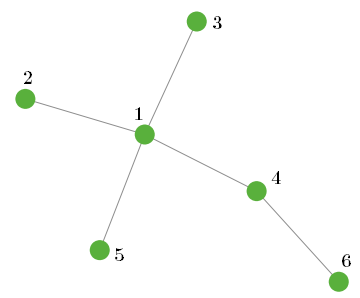
\includegraphics[width=0.5\linewidth]{../Figures/stability/Unefficientbutstablestar.png}
  \caption{\label{fig:stablestar} The resulting network after a simulation with the parameters from table \ref{tbl:stablestar} .}
\end{figure}
As we see this is not an efficient star, but the network is stable. The efficient network would be to delete the link $4,6$ and adding the link $1,6$. But since we only consider a link at a time this can not be done. To show this let $U_{i}$ denote the payoff of node $i$, the payoffs of the nodes are as described in eq (\ref{eq:payoffstablestar}).
\begin{eqnarray}
U_{1}=4\beta+\beta^2-4c\\
U_{2}=U_{3}=U_{5}=\beta+3\beta^2+\beta^3-c\\
U_{4}=2\beta+3\beta^2-2c\\
U_{6}=\beta+\beta^2+3\beta^3-c
\label{eq:payoffstablestar}
\end{eqnarray}
Node $6$ would benefit from adding the link $1,6$, but node 1 is not willing to do so because then he must pay an extra cost, and since $\beta^2>\beta-c$. Thus the network is stable but not efficient. 
In the paper \cite{jackson2005survey} they come up with this proposition:
Consider the symmetric connections model in the case where $\beta-beta^2<c<\beta$. As the number of nodes grows, the probability that a stable state (under the
process where each link has an equal probability of being identified) is reached with the
efficient network structure of a star goes to 0.
We confirmed this when running multiple simulations, when we used few nodes the resulting network often became a star, but as the number of nodes increased the network rarely was a star.
However, the structure of the networks are very similar to a scale-free network. There are many nodes with low node degree, and few with a high node degree.
One example of this is shown in figure \ref{fig:stablescalefree}, there are only ten nodes, but the network have the properties of a scale-free. Two nodes with degree of 4, and the rest have a degree of one or two.
\begin{figure}[h]
\centering
  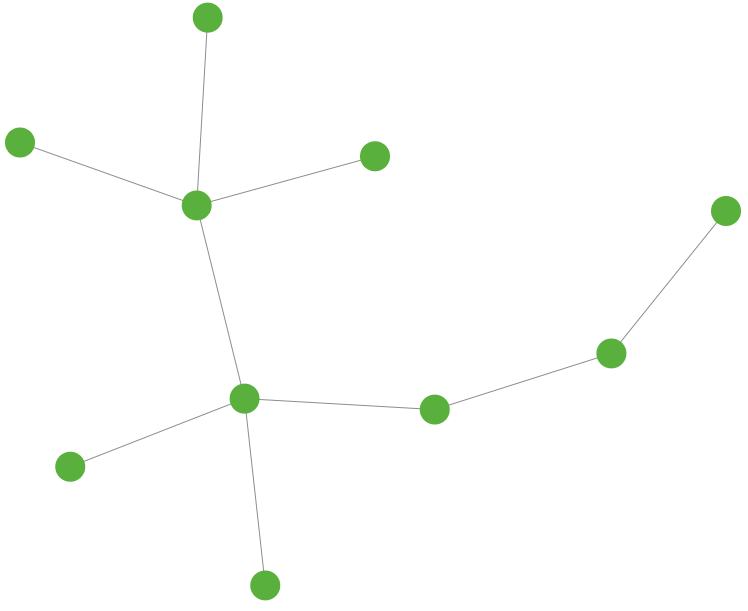
\includegraphics[width=0.5\linewidth]{../Figures/stability/Unefficientbutstabletwo.png}
  \caption{\label{fig:stablescalefree} The resulting network after a simulation with the parameters from table \ref{tbl:stablestar} and ten nodes.}
\end{figure}
\subparagraph{Bulk insurance}
As noted before it is not preferable to be the center node, due to the cost of all the direct links. If we consider the model with bulk insurance discount, this would lower the extra cost for the center node significantly. This could be used to increase the probability of reaching a star formation. One problem with this could be that if the incentive of having many connections are to good, then every would suddenly want to be a hub, and thus the incentive would defeat its purpose. 

Using the discount formula from the previous model, we end up with the equation (eq \ref{eq:discountstar}) to achieve a efficient and stable star topology. $i$ represents the node degree.
\begin{equation}
\beta-\beta^2<\frac{i_{l}}{i+1}< \beta
\label{eq:discountstar}
\end{equation}
An interesting property of the discount model is that the conditions for a efficient networks will change. Because
if $\frac{I_{l}}{m-1}<\beta-\beta^2$ and $m$-represents the number of nodes in the network, then the most efficient network is a fully connected one, because then every node has minimized their costs and maximized their payoff.
Another possibility for solving the problem with unfair costs, could be to use a shared-network cost instead. i.e. every node pays a cost equal to the total cost of the network divided on the number of nodes. 
Similar value distribution has been analyzed by Jackson and Wolinsky in \cite{jackson1996strategic}, and is called an egalitarian allocation rule, this rule guarantees that any efficient network is also pairwise stable. But this is unfortunately a very extreme rule.






